\section{Domain Name System Security}


\paragraph{DNS}
Main function is to provide a mapping of names to resources of several types (e.g. resolving a domain name to an IP address) in a hierarchical and decentralized fashion. It is a globally distributed, loosely coupled, scalable, reliable and dynamic database. Data is maintained locally and retrieved globally.

\begin{figure}[h]
	\centering
	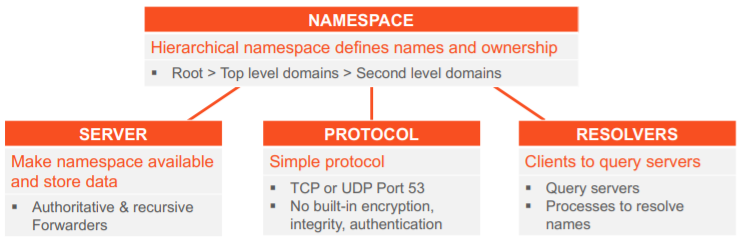
\includegraphics[scale=0.8]{images/915-dns.PNG}
	\caption{DNS key components.}
	\label{fig:dns}
\end{figure}

\paragraph{DNS Security is Critical}
Manipulating the DNS mapping allows an attacker to redirect connections, perform MITM / impersonation attacks and to launch DoS attacks. For an attacker, a DNS is a freely available distributed storage system or can be used to setup services that are hard to hunt / shut down (e.g. botnets, fast- and domain flux).

\paragraph{DNS Namespace}
A distributed global lookup mechanism for translating names into other objects organized in a hierarchy (see Figure \ref{fig:namespace}). Authoritative name servers are responsible for mapping domain names to actual Internet resources for each domain (configured by an admin). For each domain, one can define DNS zones that contain a number of distinct sub-level domains (= leaf-nodes).

\begin{figure}[h]
	\centering
	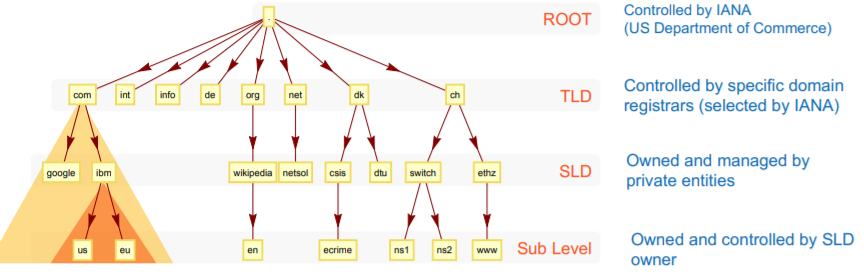
\includegraphics[scale=0.8]{images/915-namespace.PNG}
	\caption{Hierarchical DNS namespace.}
	\label{fig:namespace}
\end{figure}

\paragraph{DNS Resolution}
When a client makes a DNS request for a specific domain, it can go through many levels of delegations as depicted in Figure \ref{fig:resolution}.

\begin{figure}[h]
	\centering
	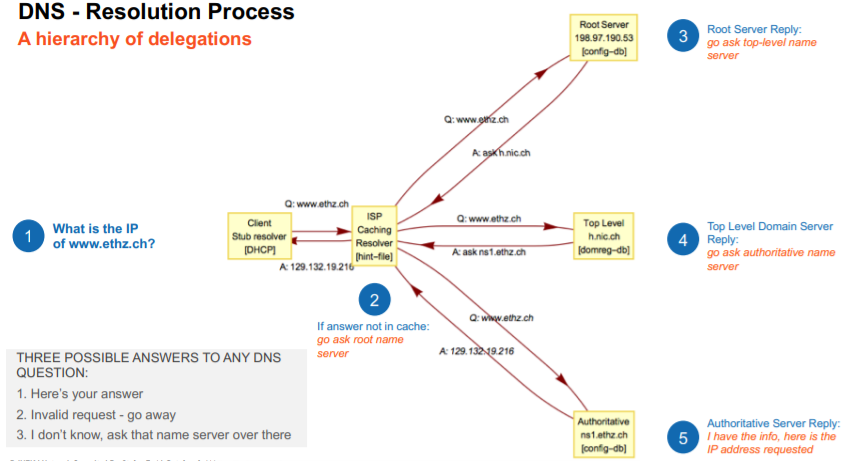
\includegraphics[scale=0.8]{images/915-resolution.PNG}
	\caption{DNS resolution process.}
	\label{fig:resolution}
\end{figure}

Resources\footnote{If a domain request couldn't be resolved in the past, it is cached with an \textit{NXDOMAIN} entry, meaning nonexistent domain.} can be cached at many points during the hierarchical query process. Cache expiration is controlled by the TTL attribute of an entry.

Requests can be resolved recursively, non-recursively or iteratively (or a combination).

\textbf{Recursive:} DNS resolver queries single DNS server which may in turn query other DNS servers. The resolver answers a query completely by querying others as needed.

\textbf{Non-recursive:} DNS resolver queries a DNS server that is either authoritative or provides a partial result.

\textbf{Iterative:} DNS resolver queries a chain of one or more DNS servers. Each server refers client to the next server on the chain until the current one can fully respond.

\paragraph{DNS Key Protocol Features}
To protect against forged responses, the first two bytes in a message form a transaction ID (\textit{txid}) that must be the same in query and response and introduces 16 bits of entropy ($2^{16}$) - it is set randomly by the client. DNS messages can either use TCP or UDP (port 53).

\textbf{Security:} If the \textit{txid} does not match, client drops response. Furthermore, client can choose a random source port (16 bits of entropy). There is no confidentiality, integrity verification nor authenticity.

\paragraph{DNS Resource Record (RR) Types}
RRs define data types in DNS. Each record has a type (name and number), a TTL, a class and type-specific data. See Figure \ref{fig:rr} for an overview of the most common ones.

\begin{figure}[h]
	\centering
	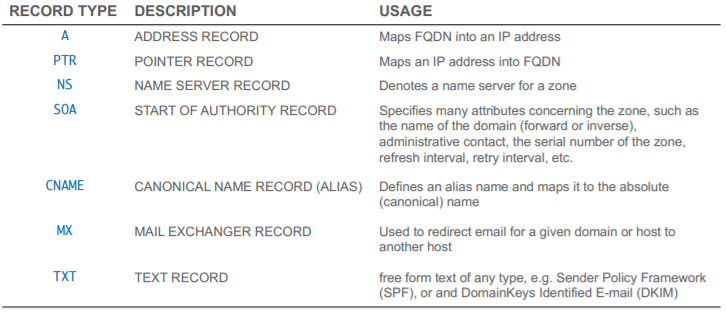
\includegraphics[scale=0.8]{images/915-rr.PNG}
	\caption{DNS resource record types.}
	\label{fig:rr}
\end{figure}

\paragraph{Attack Patterns}
Objective: insert tampered information into a DNS server or resolution process. See Figure \ref{fig:attack} for possible attacks on the DNS resolution process.

\begin{figure}[h]
	\centering
	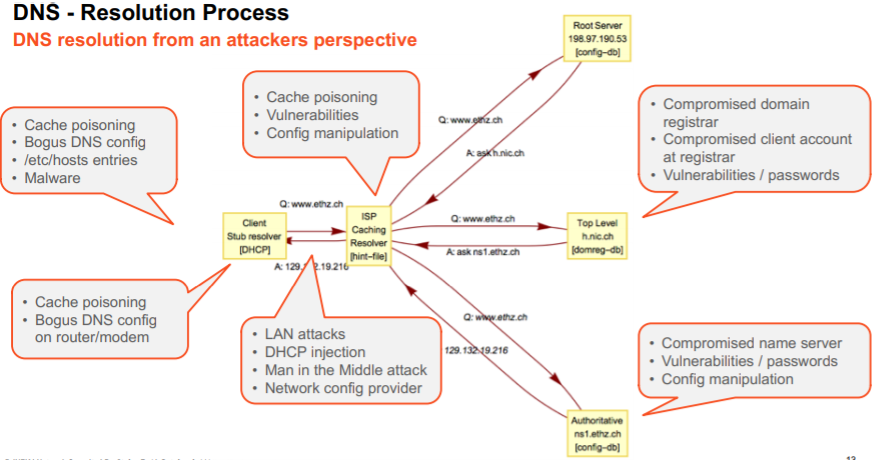
\includegraphics[scale=0.8]{images/915-attack.PNG}
	\caption{DNS resolution process from an attackers perspective.}
	\label{fig:attack}
\end{figure}

\paragraph{Common DNS Attacks}
\begin{itemize}
    \item \textbf{Local Host / Network:} Manipulate DNS entries and conversation on local host or network to impersonate services.
    \item \textbf{Cache Poisoning:} Inject manipulated information into DNS cache of resolver to impersonate services.
    \item \textbf{DNS Tunneling:} Use DNS as a covert communication channel to bypass firewalls to exfiltrate data and hidden communication.
    \item \textbf{DNS Hijacking:} Modify DNS record settings (often at domain registrar) to point to a rogue DNS server / domain to impersonate services.
    \item \textbf{Distributed Reflection:} Abuse a large number of DNS servers to combine reflection and amplification of queries that results in a (D)DoS attack.
\end{itemize}

\paragraph{DNS Root Server Security}
Served by 12 root server clusters (A to M) which are authoritative for queries for the top level domains. Every name resolution passes through this.

The root server system (RSS) consists of 1'342 instances and is operated by the 12 independent and diverse (globally and admin) root server operators (RSO). The primary concerns are availability and data integrity of the root zone.

To mitigate a (D)DoS attack on the network bandwidth level, hundreds of root servers are deployed accross different ISPs around the world and they're heavily anycasted.

To mitigate a (D)DoS attack on the memory / CPU level, the RSS is replicated and monitored. DNS enhancements pose a challenge (additional computational overhead).

\paragraph{Cache Poisoning}
Attacker inserts incorrect resolution information at any level of the resolution process (resolver, forwarder, etc.) and delays the reply of an authoritative name server (expensive lookup or DoS). 

It is basically a guessing game for the attacker. An attacker can force a server lookup for a domain (or multiple) and immediately send a number of fake replies that all guess the \textit{txid} and source port number of the request and include a redirect to a malicious IP.

E.g.: Vulnerability patched in 1997 - exploiting the additional section field. By tricking a client to resolve a malicious domain (attacker owns domain), the reply can include unrelated information in an \textit{additional section} field for another valid domain which is then accepted and cached.

E.g.: SADDNS Attack. By forcing a server to send out a query, its source port is public info. Using a port scanner, one can identify the open port (dropped packet = open port, else ICMP port unreachable). Once identified, send large number of spoofed DNS replies to bruteforce \textit{txid} (all while delaying the legit response). %TODO: 2020 reload, overcoming ICMP rate limits, defenses

\paragraph{Compromised Configuration}
Attacking the domain registrar and making it provision wrong information. Second level domains are registered with one of the domain registrars of the top level domain. The DNS info is as secure as the webapp / registration processes / passwords of the registrar and the domain owner.

One can also manipulate the DNS configuration settings on an internal network or local host by attacking routers, attacking DHCP exchange, using malware to change local hosts file, etc.

%TODO: lessons learned?

\paragraph{DNS Security Extensions (DNSSEC)}
An extension to DNS introduced around 2000 (slow adoption) that provides origin authentication, authenticated denial of existence, integrity but neither availability nor data confidentiality. Zone data is digitally signed using a private key for that zone (parent signs children's public keys). A resolver only needs to know the root public key to authenticate DNS messages. Can have more (list of trust anchors) for zones it trusts implicitly.

To make this work, registrants that are responsible for publishing DNS information must ensure that their data is DNSSEC signed and network operators need to enable DNSSEC validation on their resolvers.

See Figure \ref{fig:dnssec} for some resource record types introduced by DNSSEC.

\begin{figure}[h]
	\centering
	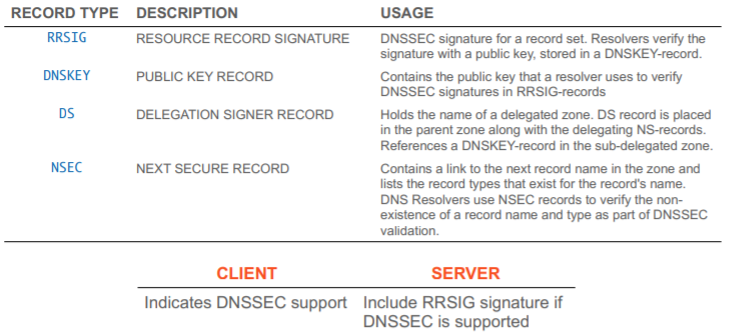
\includegraphics[scale=0.8]{images/915-dnssec.PNG}
	\caption{Resource record types added by DNSSEC.}
	\label{fig:dnssec}
\end{figure}

%TODO: disadvantages

\paragraph{DNS over HTTPS / TLS (DoH / DoT)}
Both protocols add confidentiality to DNS. Traditional DNS requests can be used to track a user. %TODO: more?


\paragraph{Conclusion}
\begin{itemize}
    \item DNS has suffered a feature creep, picking up increasingly more responsibilities.
    \item Ensure large enough randomness / entropy for critical fields.
    \item Consider impact of input validation, rate limiting, max. open / outstanding connections.
\end{itemize}